\documentclass[../../../../dd.tex]{subfiles}

\begin{document}

	\section{Component Interfaces}
	On this section we describe the interfaces of all the component of the system. The interfaces describe all the public methods that can be call to access to the components functionality.
		
		\subsection{Database Manager Component}
		\begin{figure}[H]
				\centering
				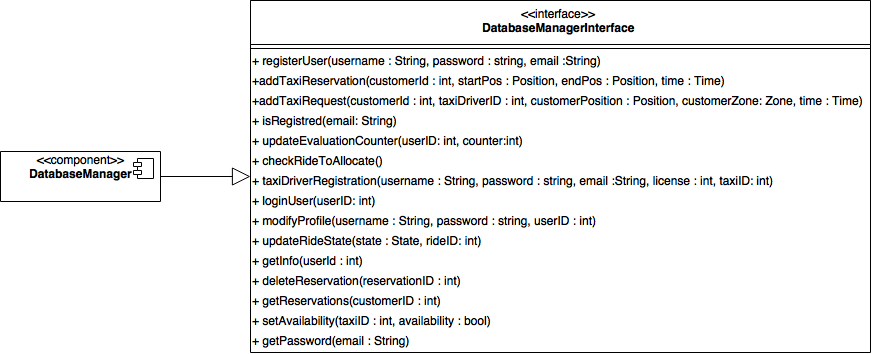
\includegraphics[width=\textwidth, scale=0.5]{../images/DatabaseManagerComponent.png}
			\caption{Database Manager Component}\label{fig:DBMSC}
		\end{figure}
		
		\subsection{Profile Manager Component}
		\begin{figure}[H]
				\centering
				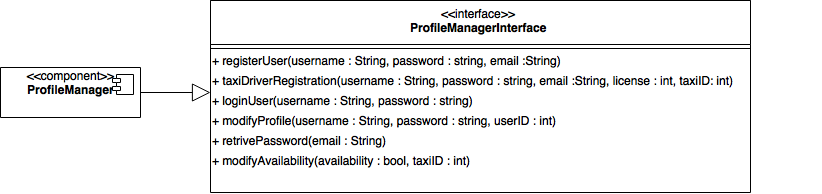
\includegraphics[width=\textwidth, scale=0.5]{../images/ProfileManagerComponent.png}
			\caption{Profile manager component}\label{fig:PMC}
		\end{figure}
		
		\subsection{IO Manager Component}
		\begin{figure}[H]
				\centering
				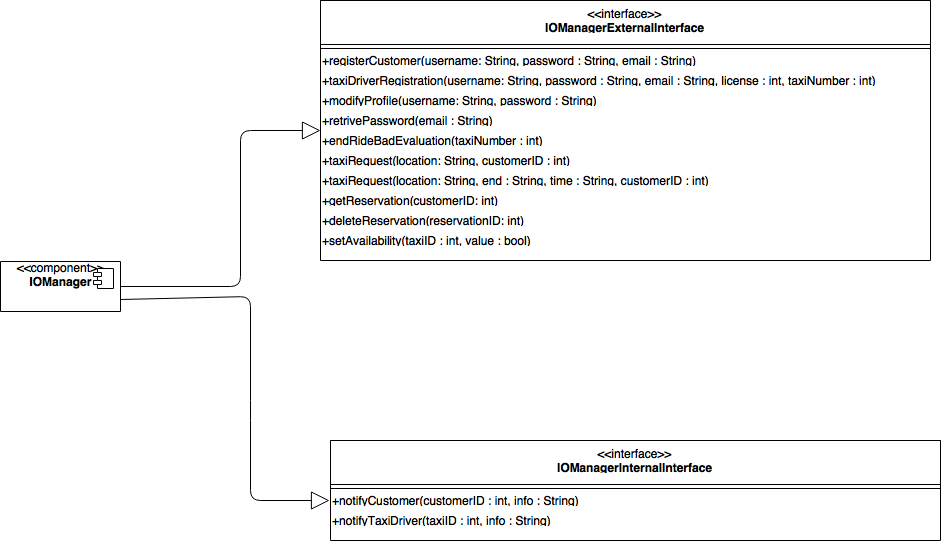
\includegraphics[width=\textwidth, scale=0.5]{../images/IOManagerComponent.png}
			\caption{IO Manager Component}\label{fig:IOMC}
		\end{figure}
		Note: In this case we have two interfaces because this class is a borderline class and need two way to be accessed. The Internal interfaces contains the public method that can be called by the component of the Logic tier. The external Interfaces can be called by all the external tiers.
	
	\subsection{Request And Reservation Manager Component}
	\begin{figure}[H]
				\centering
				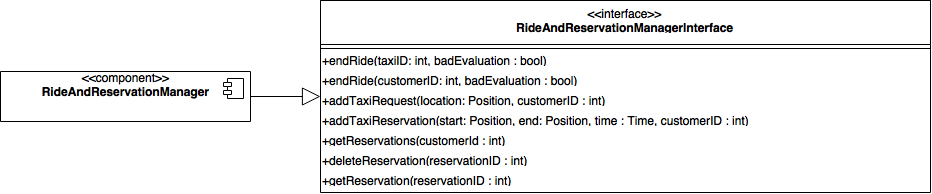
\includegraphics[width=\textwidth, scale=0.5]{../images/RequestAndReservationManager.png}
			\caption{Reservation and Request Manager Component}\label{fig:RARMC}
		\end{figure}
		
		\subsection{Zone Manager Component}
		\begin{figure}[H]
				\centering
				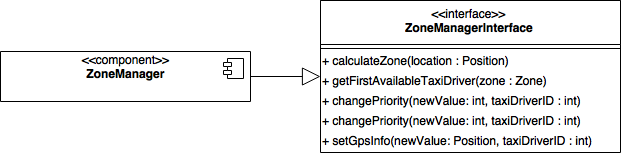
\includegraphics[width=\textwidth, scale=0.5]{../images/ZoneManagerComponent.png}
			\caption{Zone Manager Component}\label{fig:ZMC}
		\end{figure}
		
		\subsection{Presentation Tier Component}
		All the components that are present on the Presentation tier have no specific interfaces, the interfaces change for the type of visualization. We refer at their methods in an intuitive way in this document. For example if we want to open a page, we call the Open() methods, that will response with a Show() methods followed by the page that is required.
		
\end{document}